\documentclass[letter]{ieice}
\usepackage{balance}
\usepackage{flushend}
\usepackage[ruled,linesnumbered]{algorithm2e}
\usepackage{amssymb,amsthm,amsmath}
\usepackage{balance}
\usepackage{graphicx}          % graphicx package for including ps files  
\usepackage{epsfig}
\usepackage{url}
\usepackage{subfigure}
\usepackage{algorithmic}
\usepackage{float}
\newtheorem{theorem}{Theorem}[section]
\newtheorem{lemma}[theorem]{Lemma}
\usepackage{latexsym}
\usepackage{multirow}
\usepackage{color}
\usepackage{url}
\usepackage{comment}
%\usepackage{pstricks}
\usepackage{array}
\usepackage{epstopdf}
\newcolumntype{L}[1]{>{\raggedright\let\newline\\\arraybackslash\hspace{0pt}}m{#1}}
\newcolumntype{C}[1]{>{\centering\let\newline\\\arraybackslash\hspace{0pt}}m{#1}}
\newcolumntype{R}[1]{>{\raggedleft\let\newline\\\arraybackslash\hspace{0pt}}m{#1}}

\setcounter{page}{1}
%\breakauthorline{}% breaks lines after the n-th author

\field{D}
\title{SEDONA: A Novel Protocol for Identifying Infrequent, Long-Running Daemons on a Linux System}
\titlenote{This work was in part supported by the EDISON program (NRF-2011-0020576). The author acknowledges Prof. Rick Snodgrass for his suggestions to improve this article.}
\authorlist{
 \authorentry[yksuh@kisti.re.kr (Corresponding author)]{Young-Kyoon SUH}{m}{labelA}
 %\authorentry[rts@cs.arizona.edu]{Richard T. Snodgrass}{n}{labelB}}
\affiliate[labelA]{Dept. of Scientific Platform Development, Korea Inst. of Sci. and Tech. Info. (KISTI), Daejeon, 34141, Korea}
%\affiliate[labelB]{Department of Computer Science, University of Arizona, Tucson, AZ 85721, USA}
}
\received{2017}{4}{7}

\definecolor{grey}{RGB}{200,200,200}
\newcommand{\hilite}[1]{\colorbox{grey}{#1}}
\newcommand{\hilitey}[1]{\colorbox{yellow}{#1}}
\newcommand{\hiliting}[1]{\colorbox{grey}{#1}}
\long\def\todo#1{\hilitey{{\bf TODO:} {\em #1}}}
\long\def\shorten#1{}
\long\def\comment#1{}

\begin{document}

\maketitle

\begin{summary}
Measuring program execution time is 
a \hbox{much-used} technique for performance evaluation in computer science. 
Without proper care, however, timed results may vary a lot, 
thus making it hard to trust their validity. 
{\color{blue}We propose a novel timing protocol to significantly 
reduce such variability by eliminating executions involving infrequent, \hbox{long-running} daemons.}

\end{summary}
\begin{keywords}
Infrequent Long-running Daemon, Execution-Time Measurement
\end{keywords}

\vspace{-0.05in}

\section{Introduction}
\label{sec:intro}
\vspace{-0.05in}

Measuring program execution time is a much-used
technique for performance evaluation in computer science. 
Despite the importance of accurate and precise execution-time measurement, 
how to achieve {\em better} timing has not been well addressed. 
Surprisingly, there is considerable variability in the measured time.
The goal of this paper is to propose
a better timing protocol that can significantly reduce such variability 
and thus enable better timing results without a doubt of their validity.

{\color{blue}
Fig.~\ref{fig:synprog_test} compares the performance of 
the existing timing scheme, termed {\em ORG}, using elapsed time and our timing protocol, termed {\em \hbox{SEDONA}} 
(\hbox{Selective} \hbox{Elimination} through Detection of infrequent, \hbox{lOng-ruNning} dAemons), 
to be proposed shortly. 
For this comparison we used 
two kinds of real-world programs, specifically insertion sort, termed SORT and 
matrix multiplication (in column major), termed MM. 
As illustrated in Fig.~\ref{fig:synprog_test}, 
SEDONA outperformed ORG with regard to measurement quality by standard deviation. 
To be more specific, we observed that as workload size increased the performance gap between the two methods also increased, 
reaching up to by six~times. 
}

\begin{figure}[t]
	\centering
	\subfigure[SORT - Standard Deviation]{
		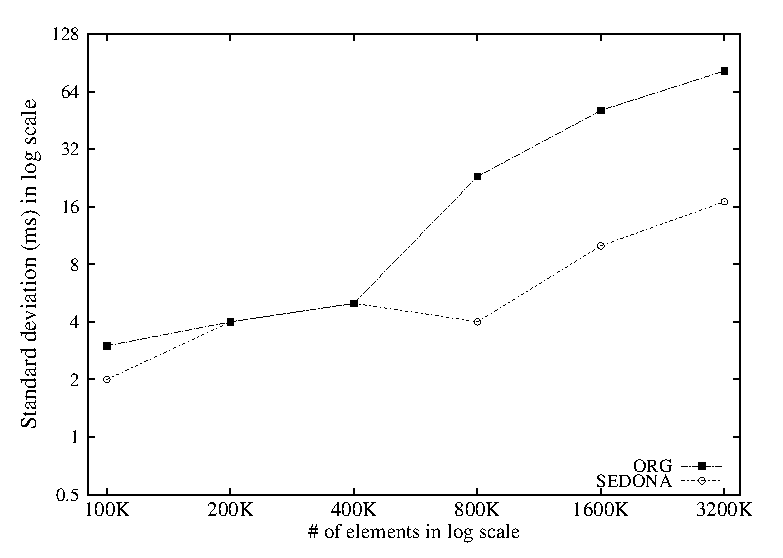
\includegraphics[scale=0.31]{sort_std.eps}
		\label{fig:sort_std}
	}
	\subfigure[MM - Standard Deviation]{
		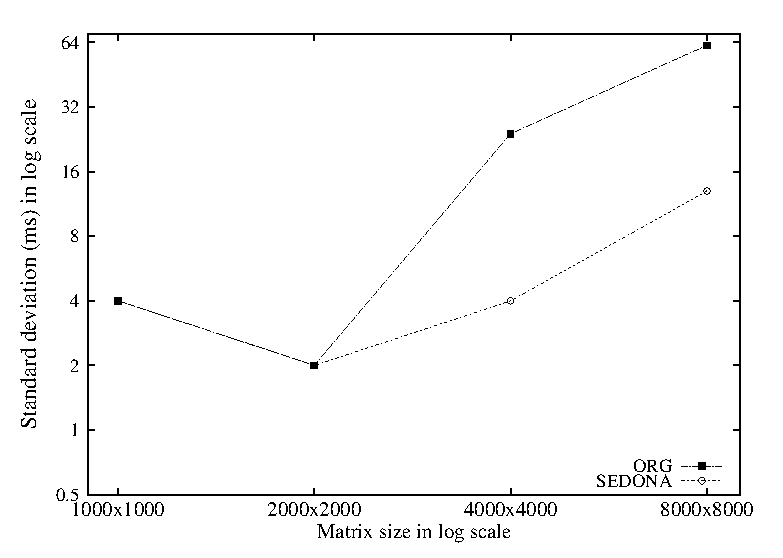
\includegraphics[scale=0.31]{matc_std.eps}
		\label{fig:matc_std}
	}
	\vspace{-.15in}
	\caption{Performance Comparison on Real-world Programs~\label{fig:synprog_test}}
\vspace{-.25in}
\end{figure}

%\vspace{-0.15in}
{\bf Characteristics.} There are several important specifics of our protocol. 
First, we utilize {\em process time} (PT) rather than on elapsed time (ET). 
The use of PT is preferred, as it takes into account 
the time taken for only a ``process'' (or program) of interest.
PT is defined as the sum of ticks (where one tick is equal to 10 msec)
in user and system mode. 
These tick measures are obtainable via {\tt taskstats} C struct, 
provided by the Linux NetLink facility~\cite{Netlink}. 
Second, the protocol throws out some executions that involve
{\em infrequent, \hbox{long-running} daemon processes}. 
We witness that such daemon processes substantially impact 
the execution time of the process.  
By eliminating those executions, the protocol greatly improves
the overall measurement quality, which would otherwise be biased by them.

{\bf Related Work.} 
McGeoch introduced
two basic methods of measuring program time: elapsed time and CPU time~\cite{Mcgeoch12}. 
Bryant and O'Hallaron~\cite{Randal03} 
presented two timing schemes of using clock-cycle and interval counters. 
They proposed a measurement protocol, called {\em minimum-of-k}, 
that for observed elapsed ticks the minimum is chosen as the most accurate one. 
Odom et al.'s work~\cite{Odom05} focused on timing long-running programs 
in a simulation framework via dynamic sampling of trace snippets during program execution. 
But none of these prior works considers the variability in 
timing and the impact of daemons that may disturb the timing a lot.

Commercial software tools measure execution time~\cite{VTune,TimeSys,WindView}. 
Since the tools' source code is not disclosed, there is no way of figuring out 
whether they can prevent such a daemon from timing. 

%\vspace{0.02in}
{\bf Contribution.} 
Our contributions are following.
\vspace{-0.05in}
\begin{itemize}

\item We show empirical evidence that 
measuring execution time 
can be seriously affected by daemons.

{\color{blue}
%\item We present an algorithm to identify infrequent, long-running daemons impacting 
%the timing of a compute-bound program.

\item We present an algorithm to identify and eliminate such daemons that are infrequent, \hbox{long-running} 
and thus impact the timing of a given program.

\item We propose a novel timing protocol that can considerably 
reduce variance via the elimination. 

\item An evaluation on real-world programs 
shows a support for the effectiveness of the protocol. 
}

\end{itemize}
\vspace{-0.05in}

\noindent
The rest is organized as follows. 
We next elaborate on the proposed timing protocol. 
{\color{blue}In turn we assess the performance of the protocol using a popular industrial benchmark suite. 
%Finally, we conclude this letter by summarizing our discussion on the proposed protocol.}
Finally, we summarize our discussion.}

\section{Proposed Scheme}
\label{sec:prop_appach}

{\color{blue}
In this section we propose our timing protocol. 
The protocol (1) utilizes PT (process time) to avoid absorbing timing noise from other co-running processes and (2)~identifies and eliminates executions including daemon processes that are infrequent and \hbox{long-running} via a {\em cutoff} measure. 

Our SEDONA protocol consists of the three major steps, as described in Fig.~\ref{alg:find}. 
Note that this protocol (algorithm) is applicable to any arbitrary Linux system and to any compute-bound program.
}

\vspace{-0.2in}
\begin{figure}[h]
\begin{center}
\begin{algorithmic}
{\bf Algorithm} The SEDONA Timing Protocol: \\
{\color{blue}
\STATE {\bf Step~A. Set up the timing environment.}
\STATE {\bf Step~B. Determine the cutoffs.}
\STATE  \ B-1. Perform a single run of a simple program-under-test (PUT) (specifically, PUT128) for many samples (specifically, 800).
\STATE  \ B-2. Consider each pair of elapsed time measurements to be a dual-PUT measurement and examine a scatter-plot to see if it it displays an $L$-shape.
\STATE  \ B-3. Zoom into the central cluster to ensure that it is symmetric (roughly circular).
\STATE  \ B-4. Compute the maximum and standard deviation of the process time for each daemon encountered within the central cluster samples.
\STATE  \ B-5. Identify for each sample in the $L$-shape infrequent, \hbox{long-running} daemon executions. 
\STATE  \ B-6. Determine potentially periodic daemons based on the \hbox{$L$-executions} and for each daemon compute the minimum process time from those executions identified. 
\STATE  \ B-7. Perform Steps 1--B-6 above for a single run consisting of a small number of executions (specifically, 40) of PUT16384.  
\STATE  \ B-8. Compute the cutoffs for each identified daemon. 
\STATE {\bf Step~C. Time an arbitrary compute-bound program.}
\STATE  \ C-1. Run the program ten times, collecting all the process times (PTs). 
\STATE  \ C-2. Discard any run involving daemon executions over the cutoffs.
\STATE  \ C-3. Compute the average to get the PT of that program.
}
\end{algorithmic}
\end{center}
\vspace{-0.05in}
\caption{The SEDONA Timing Protocol\label{alg:find}}
\vspace{-0.2in}
\end{figure}

%\vspace{-0.2in}
{\color{blue}
{\bf Timing configuration.} 
Step~A sets up the same timing environment as used in our prior work~\cite{Currim}, 
to eliminate known timing factors. 
The environment requires (i)~deactivating non-critical daemons, 
(ii)~switching on the Network Timing Protocol daemon,  
(iii)~turning off particular CPU features~\cite{intel15,intelSpeed15}, 
and (iv)~getting an up-to-date kernel installed.

{\bf Determining the Cutoffs.}
Step~B consists of eight sub-steps, resulting in determining 
the cutoffs for each identified infrequent, long-running daemon. 

In Step~B-1, we run a simple program-under-test (called PUT) many times, as shown in Fig.~\ref{alg:put}. 
PUT runs a nested for-loop with a specified task length ($tl$) (in seconds). 
The $tl$ value is used to compute 
the number of iterations ($t$) for which that for-loop is performed 
to reach the specified task length.
}

\begin{figure}[h]
\begin{center}
\begin{algorithmic}
{\bf Algorithm} PerformManyIncrements($tl$): \\
\STATE $t$ = $tl$ * {CONSTANT} \\
\FOR{$k$ = 1 to $t$ by 1}
	\FOR{$i$ = 1 to {UINT\_MAX}-1 by 1}
		\STATE $j$ += 1 \\
	\ENDFOR 
\ENDFOR 
\end{algorithmic}
\end{center}
\caption{Computation by a Program-Under-Test (PUT)\label{alg:put}}
\vspace{-0.25in}
\end{figure}

{\color{blue}
We assign a task length of 128~sec to PUT, termed {\em PUT128} and run PUT128 800~times.
We use 128~seconds because that is long enough to perhaps experience an infrequent daemon. 
We execute PUT128 800~times to capture infrequent daemons that perhaps run every few hours or even 
once a day.} 
Note that we collect all daemon processes as well as the PUT and their measures 
through the Netlink interface from the kernel before and after each 
timing.

Fig.~\ref{fig:reg_put128} plots all the 800 elapsed times (ETs) of the run of PUT128.
The plot clearly shows three rows; that is, 
the top and middle rows represent over a dozen of outliers far from 
the rest of the samples clustered in the bottom row. 
We will now drill down into these outliers to 
show how to reliably eliminate the indirect influence of 
some ``infrequent, \hbox{long-running} daemons'' on PT (\hbox{process} time) of the PUT.

\begin{figure}[h]
	\vspace{-0.3in} 
	\centering
	\subfigure[PUT128 with 800 Samples]{
		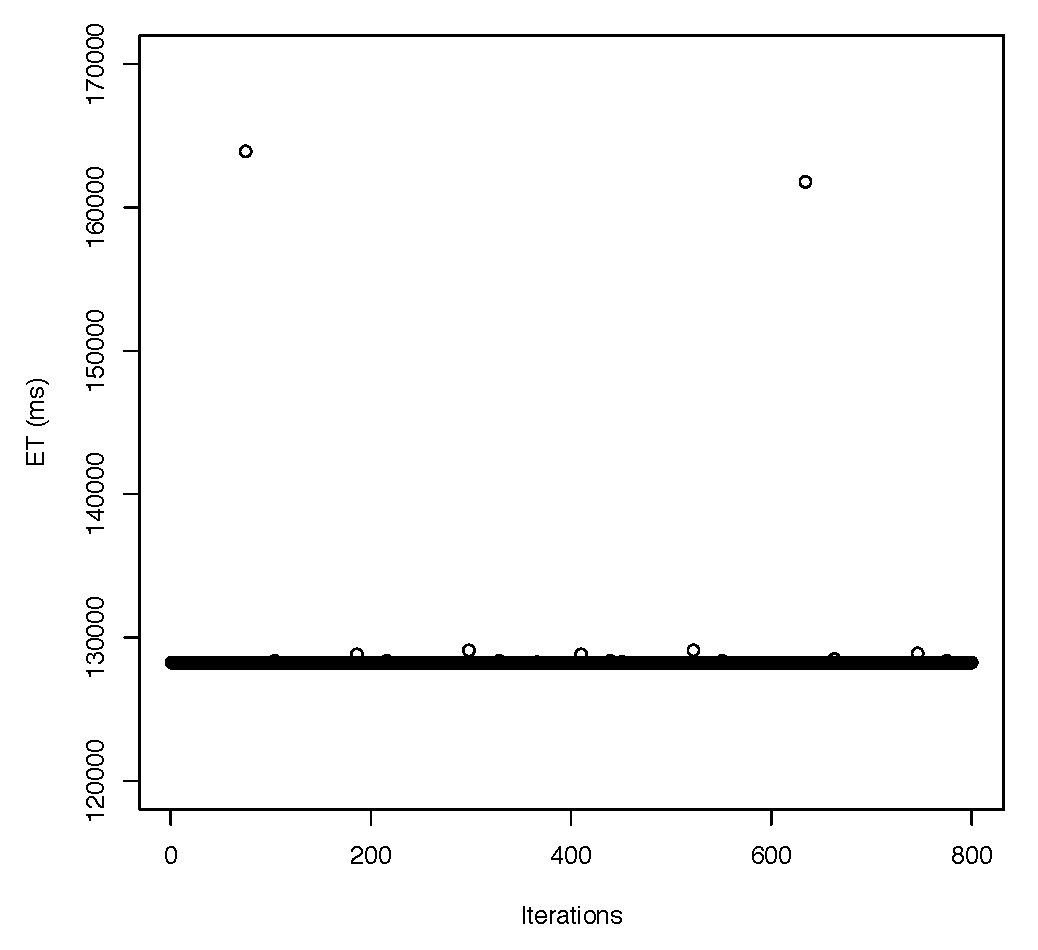
\includegraphics[width=0.224\textwidth]{put128_empv4_new.eps}
		\label{fig:reg_put128}
	}
	\subfigure[Dual-PUT256 Samples]{
		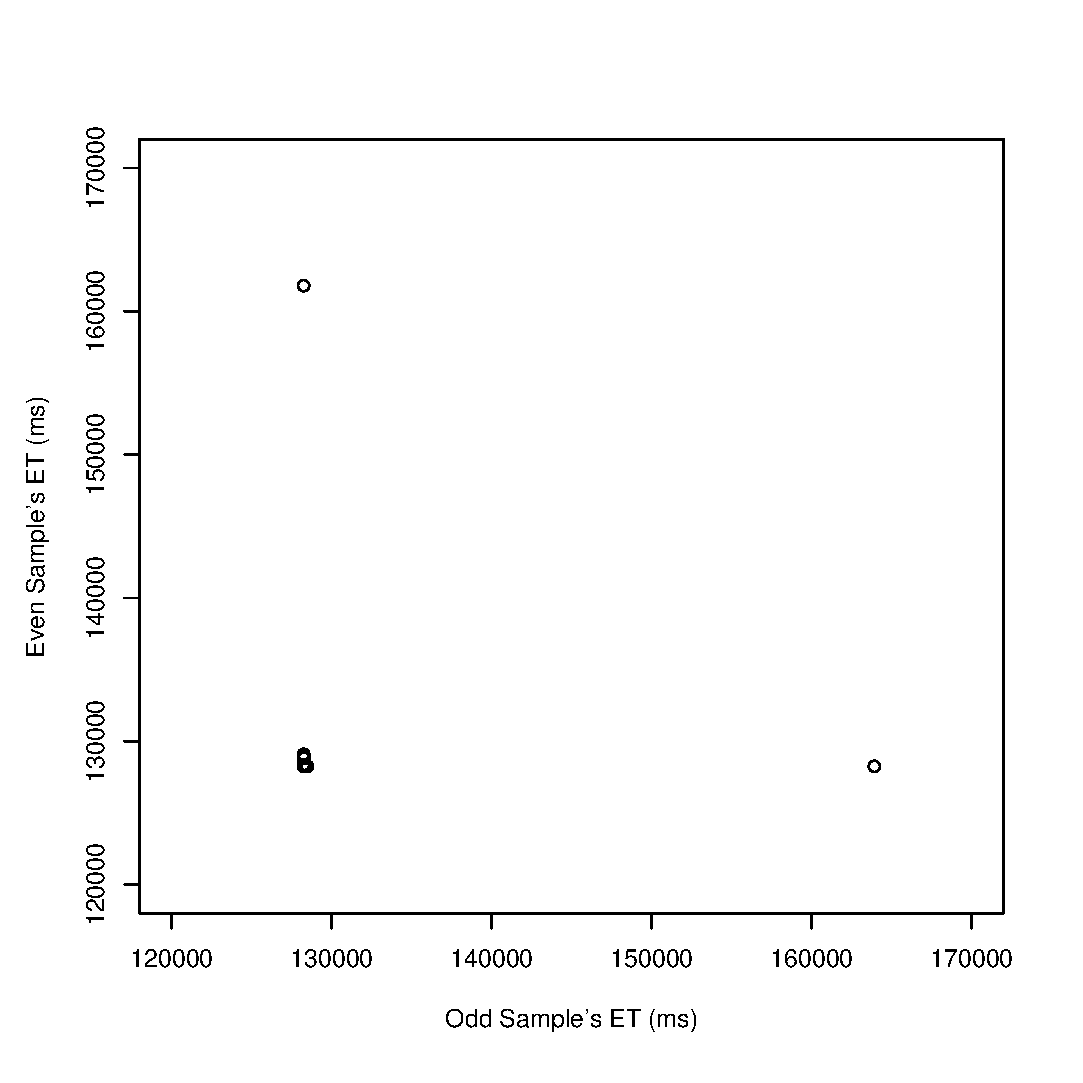
\includegraphics[width=0.224\textwidth]{dual_et_put256_empv4.eps}
		\label{fig:raw_put128}
	}\vspace{-0.15in}
	\subfigure[Zooming in on the $L$-shape]{
		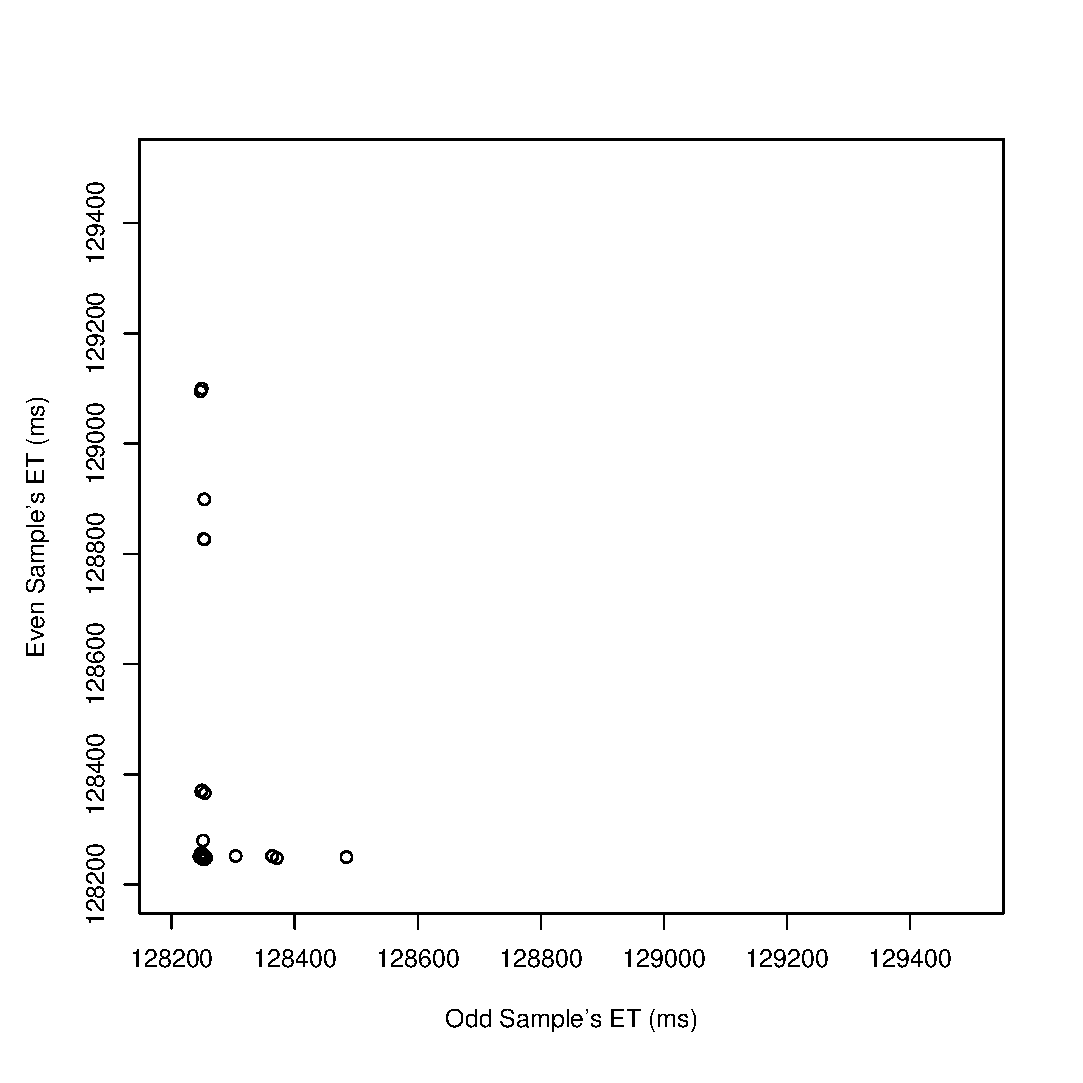
\includegraphics[width=0.224\textwidth]{zooming_in_dual_et_put256_empv4.eps}
		\label{fig:dual_put256_liters}
	}
	\subfigure[The Central Cluster]{
		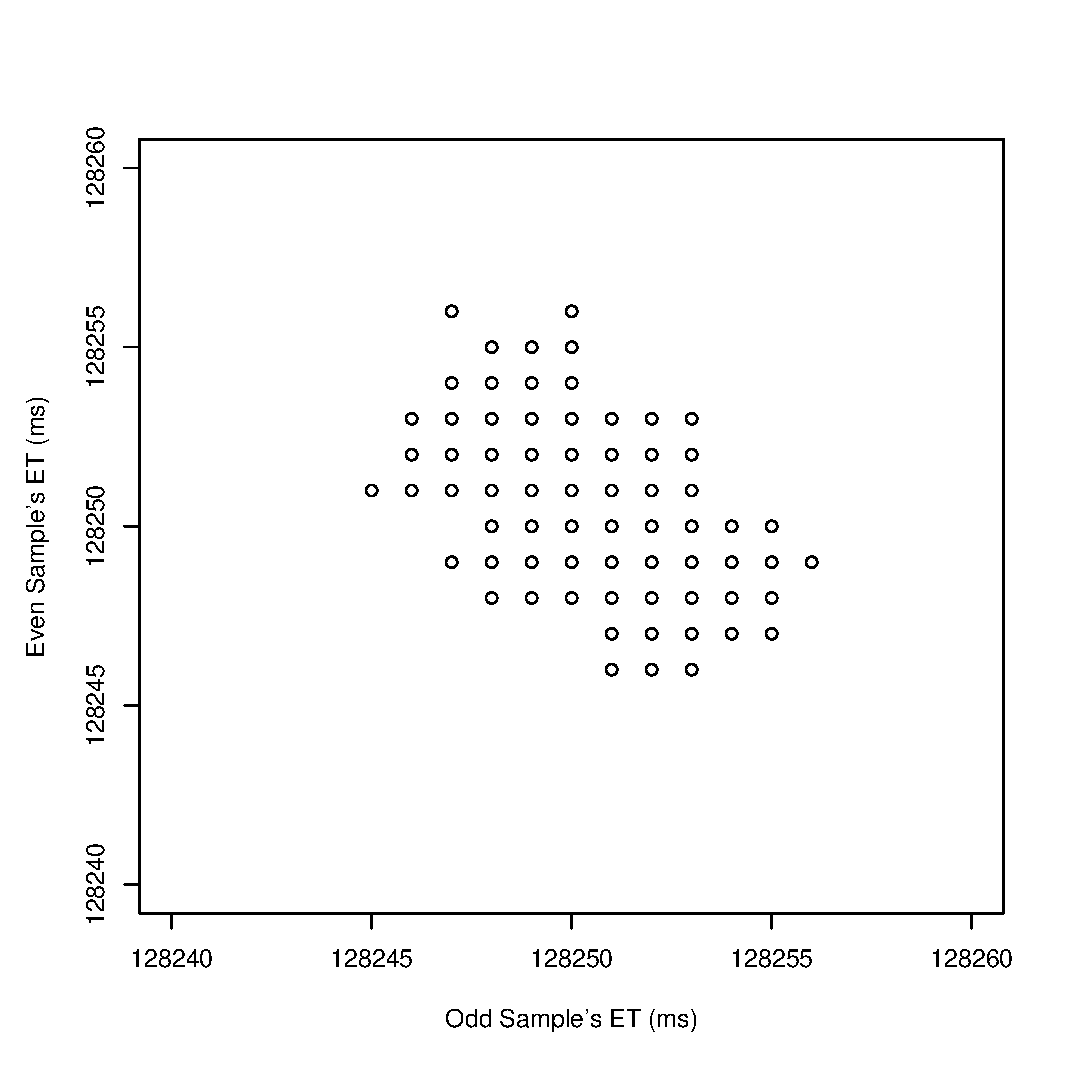
\includegraphics[width=0.224\textwidth]{dual_et_clump_put256_empv4.eps}
		\label{fig:dual_et_put256_cluster}
        }
    \caption{Successive Scatter Plots of PUT128 with 800 samples 
    (equivalent to Dual-PUT256 with 400 samples) in {\color{blue}Steps~B-1--3}~\label{fig:put128_plot}} 
    \vspace{-0.25in}     
\end{figure} 

To identify such daemons, we use a novel \hbox{scatter} plot: 
those of {\em pairs of successive samples}. 
So samples~\#{1} and~\#{2} form the first pair and samples~\#{3} and~\#{4} 
form the second pair.
Such a pair is termed ``\hbox{{\it dual-PUT}}.'' 
A sample of \hbox{dual-PUT256}, for instance, 
consists of two consecutive (odd and even) 
samples of PUT128: 
sample~\#{1} of dual-PUT256 is equivalent 
to samples~\#{1} and~\#{2} of PUT128.

Fig.~\ref{fig:raw_put128} presents such a scatter plot 
of 400 samples of a run of \hbox{dual-PUT256} constructed 
from a run of the 800 PUT128 samples ({\color{blue}Step~B-2}). 
The $xy$-plane corresponds to the dual-PUT samples. 
For example, \hbox{sample}~\#{2} of a run of dual-PUT256 
is plotted as a point with samples~\#{3} and~\#{4} of a run of PUT128 
on the respective $x$ and $y$ axes. In that sense 
the $x$ ($y$) axis is named as ``Odd (Even) Sample's ET.''
There are two quite obvious outliers with ETs 
of 163,913 ms (rightmost) and 161,785 ms (uppermost), respectively.

We informally term this phenomenon of a scatter plot of a dual-PUT run an
``$L$-shape,'' and attribute it to the
presence of infrequent long-running daemons.

Figure~\ref{fig:dual_put256_liters} zooms into the lower left region,
focusing on the
tight cluster of samples.  Interestingly, this plot continues to exhibit an
$L$-shape, with perhaps a dozen or more $L$-samples in the left and bottom arms of
the ``$L$'', and again no samples in the upper right portion of the
scatter plot.

We continue zooming until we get to Figure~\ref{fig:dual_et_put256_cluster},
which shows a central cluster ({\color{blue}Step~B-3}). 
We confirm the symmetry of the ET measurements in the central cluster: there
is no $L$-shape, and thus no $L$-samples, and thus no obvious infrequent
long-running daemons.

We then perform {\color{blue}Step~B-4}, which computes 
the maximum process time and standard deviation 
of PT (process time, note the switch in emphasis from ET to PT) of the daemon processes
(i.e. {\tt flush-9:0}) 
observed in the central cluster samples in Fig.~\ref{fig:dual_et_put256_cluster}. 

{\color{blue}Step~B-5} identifies, for each daemon in the \hbox{$L$-samples}, 
those that are actual long-running daemon
executions.  We define such executions as those whose PT 
is over two standard deviations above the maximum PT for
that daemon in the central cluster samples. 
In the running example  {\tt flush-9:0}, 
{\tt jbd2/md0-8}, and {\tt md0\_raid1} 
are determined as infrequent, \hbox{long-running}.
We also identify ``extra'' infrequent daemons: 
{\tt bash}, {\tt grep}, {\tt rhn\_check}, {\tt rhnsd}, {\tt rhsmcertd}, 
{\tt rhsmcertd-worke}, and {\tt sshd}, those 
found only in the $L$-samples but not in the central cluster. 

For each of the infrequent daemons 
we use a heuristic to determine the daemon's periodicity:
the daemon must occur regularly in a sequence of samples.
For instance, {\tt rhn\_check} appears 
roughly every 112 samples (or almost every four hours). 
Four others ({\tt flush-9:0}, {\tt jbd2/md0-8}, {\tt md0\_raid1}, and {\tt rhn\_check}) 
all occur together and have a periodicity of about every 559 samples 
(5x longer, or just about 20 hours). 

Next, we can compute for each so-identified infrequent, long-running daemon its
minimum time in the \hbox{$L$-samples} ({\color{blue}Step~B-6}). 
This computation provides a rough, initial distinction of a ``long-running''
daemon, or the valley between the maximum PT from the central cluster 
and the minimum PT from the $L$-samples, to differentiate ``short-running'' 
from ``\hbox{long-running}'' executions of the daemon. 
For those daemons (i.e. {\tt grep}) never appearing in the central cluster,
this initial \hbox{analysis} concludes only that they are infrequent.

In {\color{blue}Step~B-7} we repeat {\color{blue}Steps~1--B-6}, but instead with the much-longer running
PUT16384 (4.5 hours per \hbox{sample} versus 2 minutes), to see 
if any of our identified \hbox{infrequent} daemons are actually frequent 
at that much longer PUT execution time. 
We find some frequent daemon processes appearing in both of the 
clusters of \hbox{dual-PUT256} and \hbox{dual-PUT32768}, each consisting of 
pairs of two successive samples of PUT128 and PUT16384.
That said, the central cluster also contains other
  processes not seen in the \hbox{dual-PUT256} central cluster: 
  {\tt grep}, {\tt rhn\_check}, {\tt rhnsd}, {\tt rhsmcertd}, 
  {\tt rhsmcertd-worke}, and {\tt sshd}. 
  But these daemons were categorized in the \hbox{dual-PUT256} analysis as {\em
  infrequent}, several having \hbox{periodicities} estimated at four or twenty hours.
When PUT128 had a ``short'' 
program time (or, two minutes), daemons with a periodicity of
hours are \hbox{infrequent}. But with PUT16384 
with a ``long'' program time (or, 4.5 hours),
some of those daemons are now frequent, and appear in the central cluster.

In {\color{blue}Step~B-8} we compute 
the cutoff for each of those infrequent, long-running daemons so
identified, based on the runs of PUT128 and 
PUT16384 as collected in Tab.~\ref{tab:final_infrequent_cutoff}. 
Here is how to compute the cutoff. For the cutoff of such a daemon with PUT128, 
we take the \hbox{midpoint} between the maximum of that daemon's PTs in the 
central cluster (or 0, if absent) and the \hbox{minimum} of those in the $L$-samples. 
For the cutoff of such a daemon with PUT16384, we do the same. 
We then compute a ``task time'' as 5\% of the inferred periodicity. 
This 5\% ensures that such infrequent daemons will impact 
only a small percentage of the shorter PUTs, while presumably being 
associated with much larger cutoffs for the very long PUTs. 
We also include daemons that (a)~were identified as infrequent and 
\hbox{long-running} from PUT128 and (b)~were not identified as so in the PUT16384 
\hbox{$L$-samples}, but may have in the \hbox{dual-PUT32768} central cluster.
We then take the {\em maximum} of the two cutoffs for the final cutoff PT 
(the last column of Tab.~\ref{tab:final_infrequent_cutoff}). 
%(Note that a different distribution than RedHat Enterprise Linux may yield different cutoff data from those of Tab.~\ref{tab:final_infrequent_cutoff}, but this cutoff idea is applicable to any Linux distribution and arbitrary program.)

\vspace{-0.2in}
\begin{table}[h]
\centering
{\scriptsize
\begin{tabular}{|p{1.2cm}|p{1.2cm}|p{1.4cm}|p{1cm}|p{1.45cm}|} \hline
{\tiny Process}  & {\tiny Cutoff PT} & {\tiny Cutoff PT} & {\tiny Task}  & {\tiny{\bf Final }} \\
{\tiny Name} & {\tiny on PUT128}  & {\tiny on PUT16K} & {\tiny Time} & {\tiny {\bf Cutoff PT}} \\\hline
{\tt bash} & 1 msec & --- & --- & {\bf 1 msec} \\ \hline
{\tt flush-9:0} & 64 msec & --- & $< 1$ hour & {\bf 64 msec} \\
                & ---     & 48 msec & $\geq 1$ hour & {\bf 48 msec} \\ \hline
{\tt grep }     & 1 msec & 12 msec & --- & {\bf 12 msec}\\ \hline
{\tt jbd2/md0-8} & 4 msec & --- & $< 1$ hour & {\bf 4 msec} \\
                & ---     & 11 msec & $\geq 1$ hour & {\bf 11 msec} \\ \hline
{\tt md0\_raid1} & 35 msec & ---     & $< 1$ hour  & {\bf 35 msec}\\
                 & ---     & 51 msec & $\geq 1$ hour & {\bf 51 msec} \\ \hline
{\tt rhn\_check}  & 281 msec & --- & $< 12$ min & {\bf 281 msec} \\
                 &  --- & 12,828 msec & $\geq 12$ min & {\bf 12,828 msec}\\ \hline
{\tt rhnsd} & 2 msec & --- & $< 12$ min & {\bf 2 msec} \\
            & ---    & 12 msec &$\geq 12$ min & {\bf 12 msec} \\ \hline
{\tt rhsmcertd}  & 1 msec & 1 msec & --- & {\bf 1 msec} \\  \hline
{\tt rhsmcertd}  & 57 msec & --- & $< 12$ min & {\bf 57 msec} \\
{\tt -worke}           &  --- & 119 msec  & $\geq 12$ min & {\bf 119 msec}\\ \hline
{\tt sshd} & 2 msec & 23 msec & --- & {\bf 23 msec}\\ \hline
\end{tabular}
}
\caption{Collected Infrequent, Long-running Daemons and Their Final Cutoff
  Process Time \hbox{({\color{blue}Step~B-8})}\label{tab:final_infrequent_cutoff}}
  \vspace{-0.25in}
\end{table}

{\color{blue}
{\bf Time an arbitrary compute-bound program.} 
Step~C measures the execution time of a given program. 
In Step~C-1, we execute that program ten times~\cite{Currim}, collecting all the process times (PTs).
We then drop any execution involving daemons of which PTs are over 
their respective cutoffs in Tab.~\ref{tab:final_infrequent_cutoff} (Step~C-2).
Finally, \hbox{Step~C-3} calculates the PT of that program as the average among the retained executions' PTs.

%Now, we report the evaluation results of SEDONA. 
}

\section{Evaluation}
\label{sec:eval}
\vspace{-0.07in}
{\color{blue}
We now evaluate the \hbox{performance} of SEDONA, 
compared to that of the original timing scheme (ORG) based on elapsed time.
Our experiments were conducted on a commodity \hbox{machine}
described in Table~\ref{tab:machine_config}. 
\vspace{-0.3in}
\begin{table}[h]
\begin{center}
{\tiny
\begin{tabular}{|l|p{6.8cm}|}\hline
OS & Red Hat Ent. Linux (RHEL) 6.4 with a kernel of 2.6.32 \\ \hline
CPU & Intel Core i7-870 Lynnfield 2.93GHz quad-core \hbox{processor}\\ \hline
RAM & 4GB of DDR3 1333 dual-channel memory\\ \hline
HDD & Western Digital Caviar Black 1TB 7200rpm SATA Drive\\ \hline
\end{tabular}
}
\end{center}
\caption{Machine Configurations\label{tab:machine_config}}
\vspace{-0.3in}
\end{table}

As already seen in Figure~\ref{fig:synprog_test}, we 
confirmed the validity of our protocol with two 
real \hbox{CPU-bound} programs---insertion sort and \hbox{column-major} matrix multiplication---with heavy memory references.

To assess the performance of the protocol, 
we proceeded with SPEC CPU2006 benchmarks~\cite{specCpu2006}, providing various 
\hbox{compute-bound} real applications.
%The results are \hbox{provided} in Table~\ref{tab:spec_real}. 
%Note that in the table the results for {\tt 481} and {\tt 483} \hbox{benchmarks} 
%are omitted because of some runtime error and incurred I/O, respectively.
Note that in this evaluation we could not obtain the results for {\tt 481} and {\tt 483} \hbox{benchmarks}. 
{\tt 481} threw some runtime error that we could not resolve, and {\tt 483} incurred I/O, which was out of scope of this article.
Hence, those two results are omitted in Table~\ref{tab:spec_real}.

Consequently, we affirmed from Table~\ref{tab:spec_real} that \hbox{SEDONA} bettered ORG,
on the standard deviation and relative error across the very different SPEC benchmarks.
Specifically, all the benchmarks revealed a smaller standard deviation 
from SEDONA as compared to that of ORG.
Our timing protocol quite effectively filtered out infrequent daemon executions 
in the industrial workloads. The relative error of SEDONA was also 
lower than that of ORG for almost every benchmark.
Roughly a 10x margin between the two schemes resulted from the {\tt 434} benchmark, for instance.
}

SEDONA also scaled well for the SPEC workloads, 
with regard to growth of relative error as the execution time lengthened.
For the short benchmarks 
(e.g. {\tt 400}, {\tt 403}, {\tt 410}, 
{\tt 434}, {\tt 445}, and {\tt 999}: those taking \hbox{under} 100 sec), 
our scheme outperformed the ORG method by about 3.5x, on average. 
The SEDONA protocol continued its dominance against the conventional technique 
for the medium-length benchmarks (e.g. {\tt 447}, {\tt 456}, {\tt 470}, and {\tt 473}).
Even for the long-running benchmarks (e.g. {\tt 416}, {\tt 436}, and {\tt 454}, both $>$1,000 sec), 
the relative error of \hbox{SEDONA} was still lower than that of ORG.

To summarize, our proposed SEDONA protocol can achieve {\em better} accuracy,
precision, and scalability in measuring the execution time of real \hbox{compute-bound} programs 
than the ET-based existing method. 
The experimental results demonstrate 
the general applicability of SEDONA to timing any CPU-bound program.

\begin{table}[t]
\centering
{\tiny
\begin{tabular}{|p{0.1cm}|R{1.1cm}|R{1.1cm}|R{0.6cm}|R{0.6cm}|R{0.92cm}|R{0.92cm}|} \hline
 		  & \multicolumn{2}{c|}{{\tiny Execution Time (ms)}} & \multicolumn{2}{c|}{{\tiny Standard}}   & \multicolumn{2}{c|}{\multirow{2}{*}{{\tiny Relative Error}}}\\ \cline{2-3}
 & \multicolumn{1}{c|}{{\tiny{ORG}}}  & \multicolumn{1}{c|}{{\tiny{SED.}}} & \multicolumn{2}{c|}{{\tiny Deviation (ms)}}  & \multicolumn{2}{c|}{{\tiny}}\\ \cline{4-7}	
 & \multicolumn{1}{c|}{{\tiny{(in ET)}}} & \multicolumn{1}{c|}{{\tiny{(in PT)}}} & {\tiny{ORG}} & {\tiny{SED.}} & \multicolumn{1}{c|}{{\tiny{ORG}}}& \multicolumn{1}{c|}{{\tiny{SED.}}}\\ \hline
{{\tt 400}} & 454 & 445 & {3} & {2} & {6$\times$10$^{-3}$} & {3$\times$10$^{-3}$}\\
{{\tt 401}} & 536,639 & 528,517 & {1,185} & {1,161} & {2$\times$10$^{-3}$} & {2$\times$10$^{-3}$}\\
{{\tt 403}} & 26,109	& 25,695 & {138} & {96} & {5$\times$10$^{-3}$} & {4$\times$10$^{-3}$}\\
{{\tt 410}} & 7,938 & 7,801 & {46} & {19} & {6$\times$10$^{-3}$} & {2$\times$10$^{-3}$}\\
{{\tt 416}} & 1,015,342 & 999,846 & {965} & {876} & {1$\times$10$^{-3}$} & {9$\times$10$^{-4}$}\\%% V
{{\tt 429}} & 235,811 & 232,209 & {623} & {600} & {3$\times$10$^{-3}$} & {3$\times$10$^{-3}$}\\
{{\tt 433}} & 480,586 & 473,256  & {743} & {725} & {2$\times$10$^{-3}$} & {2$\times$10$^{-3}$}\\ %% V
{{\tt 434}} & 16,495  & 16,242  & {75} & {7} & {5$\times$10$^{-3}$} & {5$\times$10$^{-4}$}\\
{{\tt 435}} & 990,575 & 975,445  & {947} & {900} & {1$\times$10$^{-3}$} & {9$\times$10$^{-4}$}\\
{{\tt 436}} & 1,160,742 & 1,143,078   & {3,914} & {3,843} & {3$\times$10$^{-3}$} & {3$\times$10$^{-3}$}\\
{{\tt 437}} & 581,635 & 572,775 & {1,492} & {1,475}  & {3$\times$10$^{-3}$} & {3$\times$10$^{-3}$}\\
{{\tt 444}} & 591,201 & 582,229 & {294} & {281}  & {5$\times$10$^{-4}$} & {5$\times$10$^{-4}$}\\
{{\tt 445}} & 84,435  & 83,164  & {91} & {28}  & {1$\times$10$^{-3}$} & {3$\times$10$^{-4}$}\\
{{\tt 447}} & 521,846 & 513,493  & {150} & {108}  & {3$\times$10$^{-4}$} & {2$\times$10$^{-4}$}\\
{{\tt 450}} & 341,030 & 335,848  & {99} & {91}  & {3$\times$10$^{-4}$} & {2$\times$10$^{-4}$}\\
{{\tt 453}} & 258,797 & 254,496  & {623} & {582}  & {2$\times$10$^{-3}$} & {2$\times$10$^{-3}$}\\
{{\tt 454}} & 1,721,804 & 1,695,613  & {678} & {627}  & {4$\times$10$^{-4}$} & {4$\times$10$^{-4}$}\\
{{\tt 456}} & 410,533 & 404,328  & {85} & {50}  & {2$\times$10$^{-4}$} & {1$\times$10$^{-4}$}\\
{{\tt 458}} & 589,541 & 580,591  & {542} & {513} &  {9$\times$10$^{-4}$} & {9$\times$10$^{-4}$}\\
{{\tt 459}} & 798,917 & 786,726  & {2,143} & {2,132}  & {3$\times$10$^{-3}$} & {3$\times$10$^{-3}$}\\
{{\tt 462}} & 595,188 & 586,120  & {3,326} & {3,274}  & {6$\times$10$^{-3}$} & {6$\times$10$^{-3}$}\\
{{\tt 464}} & 649,838 & 639,939  & {601} & {563}  & {9$\times$10$^{-4}$} & {9$\times$10$^{-4}$}\\
{{\tt 465}} & 895,754 & 882,106  & {883} & {797}  & {1$\times$10$^{-3}$} & {1$\times$10$^{-3}$}\\
{{\tt 470}}	& 349,830 & 344,510 & {143} & {94} & {4$\times$10$^{-4}$} & {3$\times$10$^{-4}$}\\
{{\tt 471}} & 367,589 & 361,959  & {2,114} & {2,072} & {6$\times$10$^{-4}$} & {6$\times$10$^{-4}$}\\
{{\tt 473}} & 362,587 & 357,090  & {359} & {317} &  {1$\times$10$^{-3}$} & {9$\times$10$^{-4}$}\\
%{{\tt 481}} & \multicolumn{4}{c}{Runtime Error}\\
{{\tt 482}} & 654,208	 & 644,223  & {2,436} & {2,392} &   {4$\times$10$^{-3}$} & {4$\times$10$^{-3}$}\\ %% V
%{{\tt 483}} & \multicolumn{4}{c}{Out-of-Scope}\\
{{\tt 998}} & 128	 & 127  & {0.6} & {0.6} &  {4$\times$10$^{-3}$} & {4$\times$10$^{-3}$}\\
{{\tt 999}} & 128 &  127 & {0.8} & {0.6} &  {6$\times$10$^{-3}$} & {5$\times$10$^{-3}$}\\ \hline 
\multicolumn{3}{|r|}{Averages} & 852 & 815 &  {3$\times$10$^{-3}$} & {2$\times$10$^{-3}$}\\ \hline
\end{tabular}
}
\caption{Performance Evaluation on the SPEC Benchmarks\label{tab:spec_real}}
\vspace{-0.3in}
\end{table}

%\vspace\fill

\section{Conclusion}
\label{sec:conclusion}
\vspace{-0.05in}

We proposed a novel timing protocol called {\em SEDONA}, and 
performed an empirical evaluation to show that 
it is more precise and accurate than the extant method. 
This protocol is generic, in that {\em any} arbitrary \hbox{CPU-bound} program 
can be timed with reduced variance on {\em any} Linux distribution, via the protocol. 

\balance

{\scriptsize
%\vspace{-0.2in}
\bibliographystyle{ieicetr} 
\bibliography{paper}
%\vspace{-0.1in}
}

\vspace\fill
\end{document}